\documentclass[12pt,a4paper]{article}
\usepackage[utf8]{inputenc}
\usepackage[T1]{fontenc}
\usepackage[portuguese]{babel}
\usepackage{graphicx}
\usepackage{geometry}
\usepackage{listings}
\usepackage{float}
\geometry{a4paper, margin=2cm}

\title{Relatório: Ontologia do Banhado do Taim}
\author{Miguel Brondani \and Lucas Pairé}
\date{\today}

\begin{document}

\maketitle

\section{Abordagem da Solução}
Este relatório descreve o desenvolvimento de uma ontologia em OWL para representar o ecossistema do Banhado do Taim e os eventos de atropelamento de fauna na rodovia BR-471. A estrutura organiza as espécies animais, trechos da rodovia, habitats e condições climáticas. 

Para o povoamento, um script Python coletou dados sobre a fauna da região diretamente da Wikipédia, garantindo o uso de espécies reais. Outro script automatizou a geração e inserção de indivíduos (instâncias) de acidentes e trechos rodoviários, aplicando restrições de cardinalidade do modelo.

\section{Modelagem da Ontologia}
A ontologia foi organizada em cinco superclasses principais: Animal, Habitat, Rodovia, CondicaoAmbiental e Evento. A classe Animal contém classes para grupos taxonômicos (Mamifero, Ave, Reptil, Anfibio), que por sua vez possuem subclasses específicas para cada espécie validada (como Capivara e Jacaré-de-papo-amarelo). O modelo define dez propriedades de objeto (ex: envolveAnimal, ocorreEm) e treze propriedades de dados (ex: kmRodovia, fluxoVeiculosHora).

Também foram aplicadas restrições de cardinalidade nas classes principais:
\begin{itemize}
    \item \textbf{EventoAtropelamento}: deve envolver exatamente 1 Animal, ocorrer em exatamente 1 TrechoRodovia, ocorrer sob exatamente 1 CondicaoClimatica, ter exatamente 1 severidadeAcidente e 1 dataHora.
    \item \textbf{TrechoRodovia}: deve pertencer a exatamente 1 Rodovia e ter exatamente 1 kmRodovia.
\end{itemize}

\vspace{8cm}
A Figura 1 apresenta a hierarquia principal das classes no Protégé.

\begin{figure}[H]
\centering
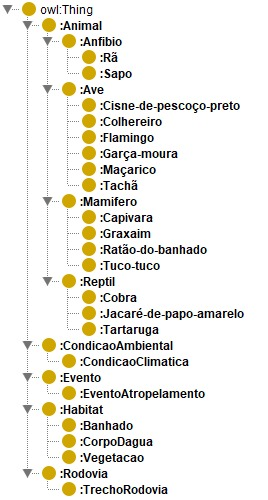
\includegraphics[width=0.4\textwidth]{images/classes.jpeg}
\caption{Hierarquia de classes no Protégé}
\end{figure}

As propriedades de objeto definem a relação entre os conceitos. A Figura 2 ilustra a interface de criação.

\begin{figure}[H]
\centering
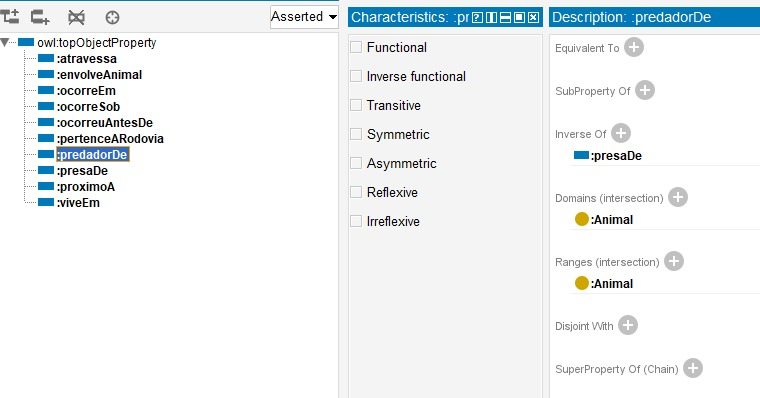
\includegraphics[width=0.8\textwidth]{images/propriedadesObjeto.jpeg}
\caption{Propriedades de Objeto}
\end{figure}

\vspace{1cm}
As propriedades de dados guardam métricas como coordenadas de GPS e temperatura. A Figura 3 mostra o mapeamento.

\begin{figure}[H]
\centering
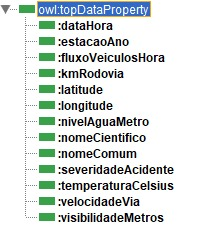
\includegraphics[width=0.4\textwidth]{images/propriedadesDados.jpeg}
\caption{Propriedades de Dados}
\end{figure}

\subsection*{Decisões de Modelagem e Alternativas Consideradas}

\textbf{Justificativa das Decisões de Modelagem:}
Os fatores de risco foram modelados diretamente como atributos (tráfego como fluxo de veículos no trecho, e visibilidade como propriedade do clima), o que simplifica o esquema de classes. A estação do ano (estacaoAno) foi incluída no evento para possibilitar buscas por período sazonal de forma direta.

\textbf{Alternativas Consideradas e Descartadas:}
\begin{enumerate}
    \item \textbf{Espécies como atributos vs. Subclasses:} Cogitou-se modelar espécies apenas como atributos de texto (ex: indivíduos da classe Mamifero com um campo nomeComum = "Capivara"). Isso foi descartado porque impedia consultas baseadas na classe específica (ex: buscar instâncias de Capivara). Definir cada espécie como uma subclasse resolveu o problema e tornou a hierarquia taxonômica correta.
    
    \item \textbf{Severidade como Classe vs. Propriedade de Dados:} Considerou-se criar uma classe própria para a severidade do acidente. A ideia foi descartada para evitar complexidade desnecessária no grafo, optando-se por um campo simples de texto no evento (ex: "Fatal", "Fuga").
\end{enumerate}

\section{Povoamento Automatizado}
O povoamento da ontologia gerou 137 indivíduos através de um script Python. O script cruzou as espécies coletadas da Wikipédia com trechos da rodovia BR-471 (KMs 10 a 29) e gerou 60 acidentes fictícios sob diferentes condições:

\begin{itemize}
    \item \textbf{Tráfego}: preenchido através da propriedade \textit{fluxoVeiculosHora} nos trechos rodoviários.
    \item \textbf{Visibilidade}: definida no clima. Dias ensolarados simulam visibilidade alta (1000m a 5000m), enquanto chuva ou neblina reduzem a visibilidade (20m a 300m).
    \item \textbf{Estação do Ano}: gerada automaticamente a partir do mês do evento (ex: Janeiro associado a "Verão", Julho a "Inverno").
\end{itemize}

A Figura 4 comprova a geração e injeção automática dos eventos de atropelamento na classe final.

\begin{figure}[H]
\centering
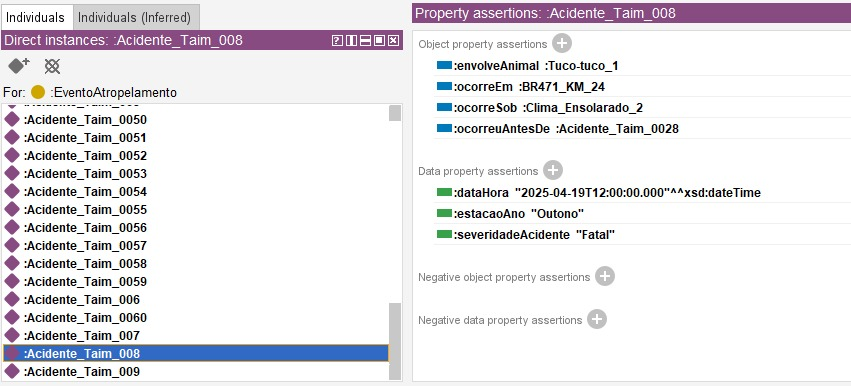
\includegraphics[width=0.8\textwidth]{images/individuos.jpeg}
\caption{Lista de indivíduos da classe EventoAtropelamento}
\end{figure}

\subsection*{Limitações e Inconsistências de Dados}
A modelagem possui algumas limitações e pontos de atenção:
\begin{itemize}
    \item \textbf{Extração de espécies}: A busca por termos na Wikipédia é baseada em palavras-chave exatas, o que pode falhar caso o texto do artigo mude ou utilize termos alternativos.
    \item \textbf{Dados simulados}: Como não há acesso fácil a uma base de dados governamental pública e atualizada de acidentes no Taim, as instâncias de atropelamento e medições climáticas foram geradas artificialmente com valores plausíveis.
    \item \textbf{Raciocínio OWL}: A biblioteca RDFLib usada em Python não executa raciocínio OWL em tempo de execução de consultas SPARQL. Para contornar isso nas buscas por superclasses (como Mamifero ou Ave), foi necessário usar caminhos de propriedades transitivas (\textit{rdf:type/rdfs:subClassOf*}) nas consultas.
\end{itemize}

\vspace{8cm}
\section{Grafo da Ontologia}
A visualização no OntoGraf apresenta a rede de conexões entre os indivíduos mapeados (animais, trechos rodoviários, climas e eventos de atropelamento), demonstrando o relacionamento entre as instâncias da ontologia.

\begin{figure}[H]
\centering
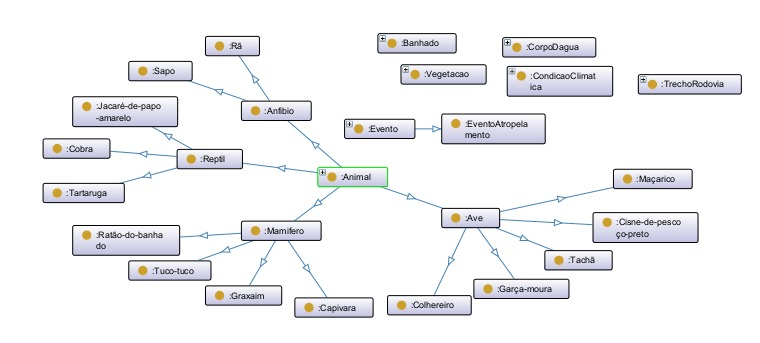
\includegraphics[width=0.8\textwidth]{images/ontologia.jpeg}
\caption{Grafo de conexões (OntoGraf)}
\end{figure}

\section{Protocolo de Uso de LLM}
Os modelos de linguagem foram utilizados como assistentes no desenvolvimento do código Python e na validação das consultas SPARQL e da sintaxe OWL. O processo seguiu três regras:
\begin{enumerate}
    \item Uso do modelo para estruturar e validar as consultas SPARQL complexas.
    \item Apoio na escrita do código de injeção e povoamento da ontologia base.
    \item Revisão das definições da ontologia para evitar erros de sintaxe.
\end{enumerate}
Nenhuma informação ecológica ou de fauna foi gerada por alucinação; todas as espécies foram estritamente validadas a partir do texto obtido da Wikipédia.

\section{Consultas SPARQL}
As trinta consultas exigidas foram automatizadas via script Python usando a biblioteca RDFLib. O código carregou o banco de conhecimento e extraiu os relatórios abaixo. As respostas comprovam a viabilidade das perguntas lógicas.

\subsection*{Categoria: Simples}

\subsubsection*{Consulta 1}

\textbf{Descrição:} Listar todas as Capivaras registradas na ontologia.

\textbf{Código SPARQL:}
\begin{lstlisting}
PREFIX rdf: <http://www.w3.org/1999/02/22-rdf-syntax-ns#>
PREFIX rdfs: <http://www.w3.org/2000/01/rdf-schema#>
PREFIX taim: <http://www.exemplo.org/taim#>
SELECT ?capivara WHERE { ?capivara rdf:type taim:Capivara . }
\end{lstlisting}

\textbf{Resultados Obtidos:}
\begin{lstlisting}
capivara: Capivara_1
capivara: Capivara_2
capivara: Capivara_3
capivara: Capivara_4
capivara: Capivara_5
\end{lstlisting}

\vspace{1cm}
\subsubsection*{Consulta 2}

\textbf{Descrição:} Listar todos os Jacarés-de-papo-amarelo registrados.

\textbf{Código SPARQL:}
\begin{lstlisting}
PREFIX rdf: <http://www.w3.org/1999/02/22-rdf-syntax-ns#>
PREFIX rdfs: <http://www.w3.org/2000/01/rdf-schema#>
PREFIX taim: <http://www.exemplo.org/taim#>
SELECT ?jacare WHERE { ?jacare rdf:type taim:Jacaré-de-papo-amarelo . }
\end{lstlisting}

\textbf{Resultados Obtidos:}
\begin{lstlisting}
jacare: Jacaré-de-papo-amarelo_1
jacare: Jacaré-de-papo-amarelo_2
jacare: Jacaré-de-papo-amarelo_3
jacare: Jacaré-de-papo-amarelo_4
jacare: Jacaré-de-papo-amarelo_5
\end{lstlisting}

\vspace{1cm}
\subsubsection*{Consulta 3}

\textbf{Descrição:} Listar todos os trechos de rodovia mapeados.

\textbf{Código SPARQL:}
\begin{lstlisting}
PREFIX rdf: <http://www.w3.org/1999/02/22-rdf-syntax-ns#>
PREFIX rdfs: <http://www.w3.org/2000/01/rdf-schema#>
PREFIX taim: <http://www.exemplo.org/taim#>
SELECT ?trecho WHERE { ?trecho rdf:type taim:TrechoRodovia . }
\end{lstlisting}

\textbf{Resultados Obtidos:}
\begin{lstlisting}
trecho: BR471_KM_10
trecho: BR471_KM_11
trecho: BR471_KM_12
trecho: BR471_KM_13
trecho: BR471_KM_14
trecho: BR471_KM_15
trecho: BR471_KM_16
trecho: BR471_KM_17
trecho: BR471_KM_18
trecho: BR471_KM_19
... (e mais 10 resultados ocultados por brevidade)
\end{lstlisting}

\vspace{1cm}
\subsubsection*{Consulta 4}

\textbf{Descrição:} Listar todos os Eventos de Atropelamento.

\textbf{Código SPARQL:}
\begin{lstlisting}
PREFIX rdf: <http://www.w3.org/1999/02/22-rdf-syntax-ns#>
PREFIX rdfs: <http://www.w3.org/2000/01/rdf-schema#>
PREFIX taim: <http://www.exemplo.org/taim#>
SELECT ?evento WHERE { ?evento rdf:type taim:EventoAtropelamento . }
\end{lstlisting}

\textbf{Resultados Obtidos:}
\begin{lstlisting}
evento: Acidente_Taim_001
evento: Acidente_Taim_002
evento: Acidente_Taim_003
evento: Acidente_Taim_004
evento: Acidente_Taim_005
evento: Acidente_Taim_006
evento: Acidente_Taim_007
evento: Acidente_Taim_008
evento: Acidente_Taim_009
evento: Acidente_Taim_0010
... (e mais 50 resultados ocultados por brevidade)
\end{lstlisting}

\vspace{1cm}
\subsubsection*{Consulta 5}

\textbf{Descrição:} Listar todas as Condições Climáticas registradas.

\textbf{Código SPARQL:}
\begin{lstlisting}
PREFIX rdf: <http://www.w3.org/1999/02/22-rdf-syntax-ns#>
PREFIX rdfs: <http://www.w3.org/2000/01/rdf-schema#>
PREFIX taim: <http://www.exemplo.org/taim#>
SELECT ?clima WHERE { ?clima rdf:type taim:CondicaoClimatica . }
\end{lstlisting}

\textbf{Resultados Obtidos:}
\begin{lstlisting}
clima: Clima_Chuva_Forte_0
clima: Clima_Neblina_Densa_1
clima: Clima_Ensolarado_2
clima: Clima_Nublado_3
\end{lstlisting}

\vspace{1cm}
\subsubsection*{Consulta 6}

\textbf{Descrição:} Listar todos os habitats do tipo Banhado.

\textbf{Código SPARQL:}
\begin{lstlisting}
PREFIX rdf: <http://www.w3.org/1999/02/22-rdf-syntax-ns#>
PREFIX rdfs: <http://www.w3.org/2000/01/rdf-schema#>
PREFIX taim: <http://www.exemplo.org/taim#>
SELECT ?banhado WHERE { ?banhado rdf:type taim:Banhado . }
\end{lstlisting}

\textbf{Resultados Obtidos:}
\begin{lstlisting}
banhado: Banhado_da_Mangueira
banhado: Banhado_do_Nicola
banhado: Banhado_Central
\end{lstlisting}

\vspace{1cm}
\subsection*{Categoria: Múltiplas Relações}

\subsubsection*{Consulta 7}

\textbf{Descrição:} Buscar eventos associados a um animal específico e o trecho onde ocorreu.

\textbf{Código SPARQL:}
\begin{lstlisting}
PREFIX rdf: <http://www.w3.org/1999/02/22-rdf-syntax-ns#>
PREFIX rdfs: <http://www.w3.org/2000/01/rdf-schema#>
PREFIX taim: <http://www.exemplo.org/taim#>
SELECT ?evento ?animal ?trecho WHERE { ?evento rdf:type taim:EventoAtropelamento . ?evento taim:envolveAnimal ?animal . ?evento taim:ocorreEm ?trecho . }
\end{lstlisting}

\textbf{Resultados Obtidos:}
\begin{lstlisting}
evento: Acidente_Taim_001 | animal: Capivara_2 | trecho: BR471_KM_23
evento: Acidente_Taim_002 | animal: Jacaré-de-papo-amarelo_1 | trecho: BR471_KM_27
evento: Acidente_Taim_003 | animal: Ratão-do-banhado_3 | trecho: BR471_KM_22
evento: Acidente_Taim_004 | animal: Cisne-de-pescoço-preto_4 | trecho: BR471_KM_11
evento: Acidente_Taim_005 | animal: Cisne-de-pescoço-preto_3 | trecho: BR471_KM_15
evento: Acidente_Taim_006 | animal: Maçarico_5 | trecho: BR471_KM_18
evento: Acidente_Taim_007 | animal: Tachã_5 | trecho: BR471_KM_16
evento: Acidente_Taim_008 | animal: Tachã_4 | trecho: BR471_KM_14
evento: Acidente_Taim_009 | animal: Capivara_3 | trecho: BR471_KM_16
evento: Acidente_Taim_0010 | animal: Jacaré-de-papo-amarelo_4 | trecho: BR471_KM_15
... (e mais 50 resultados ocultados por brevidade)
\end{lstlisting}

\vspace{1cm}
\subsubsection*{Consulta 8}

\textbf{Descrição:} Descobrir em quais habitats os animais acidentados costumam viver.

\textbf{Código SPARQL:}
\begin{lstlisting}
PREFIX rdf: <http://www.w3.org/1999/02/22-rdf-syntax-ns#>
PREFIX rdfs: <http://www.w3.org/2000/01/rdf-schema#>
PREFIX taim: <http://www.exemplo.org/taim#>
SELECT DISTINCT ?animal ?habitat WHERE { ?evento rdf:type taim:EventoAtropelamento . ?evento taim:envolveAnimal ?animal . ?animal taim:viveEm ?habitat . }
\end{lstlisting}

\textbf{Resultados Obtidos:}
\begin{lstlisting}
animal: Capivara_2 | habitat: Banhado_do_Nicola
animal: Jacaré-de-papo-amarelo_1 | habitat: Banhado_Central
animal: Ratão-do-banhado_3 | habitat: Banhado_do_Nicola
animal: Cisne-de-pescoço-preto_4 | habitat: Banhado_do_Nicola
animal: Cisne-de-pescoço-preto_3 | habitat: Banhado_da_Mangueira
animal: Maçarico_5 | habitat: Banhado_Central
animal: Tachã_5 | habitat: Banhado_Central
animal: Tachã_4 | habitat: Banhado_do_Nicola
animal: Capivara_3 | habitat: Banhado_do_Nicola
animal: Jacaré-de-papo-amarelo_4 | habitat: Banhado_do_Nicola
... (e mais 27 resultados ocultados por brevidade)
\end{lstlisting}

\vspace{1cm}
\subsubsection*{Consulta 9}

\textbf{Descrição:} Listar trechos de rodovia, seus acidentes e as condições climáticas exatas no momento.

\textbf{Código SPARQL:}
\begin{lstlisting}
PREFIX rdf: <http://www.w3.org/1999/02/22-rdf-syntax-ns#>
PREFIX rdfs: <http://www.w3.org/2000/01/rdf-schema#>
PREFIX taim: <http://www.exemplo.org/taim#>
SELECT ?trecho ?evento ?clima WHERE { ?evento taim:ocorreEm ?trecho . ?evento taim:ocorreSob ?clima . }
\end{lstlisting}

\textbf{Resultados Obtidos:}
\begin{lstlisting}
trecho: BR471_KM_23 | evento: Acidente_Taim_001 | clima: Clima_Nublado_3
trecho: BR471_KM_23 | evento: Acidente_Taim_0012 | clima: Clima_Chuva_Forte_0
trecho: BR471_KM_23 | evento: Acidente_Taim_0026 | clima: Clima_Neblina_Densa_1
trecho: BR471_KM_23 | evento: Acidente_Taim_0031 | clima: Clima_Chuva_Forte_0
trecho: BR471_KM_23 | evento: Acidente_Taim_0032 | clima: Clima_Chuva_Forte_0
trecho: BR471_KM_23 | evento: Acidente_Taim_0043 | clima: Clima_Nublado_3
trecho: BR471_KM_23 | evento: Acidente_Taim_0052 | clima: Clima_Chuva_Forte_0
trecho: BR471_KM_23 | evento: Acidente_Taim_0058 | clima: Clima_Nublado_3
trecho: BR471_KM_27 | evento: Acidente_Taim_002 | clima: Clima_Ensolarado_2
trecho: BR471_KM_27 | evento: Acidente_Taim_0025 | clima: Clima_Nublado_3
... (e mais 50 resultados ocultados por brevidade)
\end{lstlisting}

\vspace{1cm}
\subsubsection*{Consulta 10}

\textbf{Descrição:} Buscar trechos de rodovia que registraram acidentes e também estão próximos a um banhado.

\textbf{Código SPARQL:}
\begin{lstlisting}
PREFIX rdf: <http://www.w3.org/1999/02/22-rdf-syntax-ns#>
PREFIX rdfs: <http://www.w3.org/2000/01/rdf-schema#>
PREFIX taim: <http://www.exemplo.org/taim#>
SELECT ?trecho ?evento ?banhado WHERE { ?evento taim:ocorreEm ?trecho . ?trecho taim:proximoA ?banhado . ?banhado rdf:type taim:Banhado . }
\end{lstlisting}

\textbf{Resultados Obtidos:}
\begin{lstlisting}
trecho: BR471_KM_14 | evento: Acidente_Taim_008 | banhado: Banhado_da_Mangueira
trecho: BR471_KM_14 | evento: Acidente_Taim_0011 | banhado: Banhado_da_Mangueira
trecho: BR471_KM_14 | evento: Acidente_Taim_0033 | banhado: Banhado_da_Mangueira
trecho: BR471_KM_14 | evento: Acidente_Taim_0036 | banhado: Banhado_da_Mangueira
trecho: BR471_KM_21 | evento: Acidente_Taim_0016 | banhado: Banhado_da_Mangueira
trecho: BR471_KM_21 | evento: Acidente_Taim_0021 | banhado: Banhado_da_Mangueira
trecho: BR471_KM_21 | evento: Acidente_Taim_0049 | banhado: Banhado_da_Mangueira
trecho: BR471_KM_22 | evento: Acidente_Taim_003 | banhado: Banhado_da_Mangueira
trecho: BR471_KM_22 | evento: Acidente_Taim_0053 | banhado: Banhado_da_Mangueira
trecho: BR471_KM_25 | evento: Acidente_Taim_0037 | banhado: Banhado_da_Mangueira
... (e mais 50 resultados ocultados por brevidade)
\end{lstlisting}

\vspace{1cm}
\subsubsection*{Consulta 11}

\textbf{Descrição:} Listar animais que atravessaram a rodovia e se envolveram em um acidente.

\textbf{Código SPARQL:}
\begin{lstlisting}
PREFIX rdf: <http://www.w3.org/1999/02/22-rdf-syntax-ns#>
PREFIX rdfs: <http://www.w3.org/2000/01/rdf-schema#>
PREFIX taim: <http://www.exemplo.org/taim#>
SELECT ?animal ?evento WHERE { ?animal taim:atravessa ?trecho . ?evento taim:envolveAnimal ?animal . }
\end{lstlisting}

\textbf{Resultados Obtidos:}
\begin{lstlisting}
animal: Capivara_1 | evento: Acidente_Taim_0045
animal: Ratão-do-banhado_2 | evento: Acidente_Taim_0023
animal: Cisne-de-pescoço-preto_1 | evento: Acidente_Taim_0044
animal: Capivara_2 | evento: Acidente_Taim_001
animal: Capivara_5 | evento: Acidente_Taim_0052
animal: Ratão-do-banhado_3 | evento: Acidente_Taim_003
animal: Ratão-do-banhado_3 | evento: Acidente_Taim_0026
animal: Ratão-do-banhado_4 | evento: Acidente_Taim_0048
animal: Ratão-do-banhado_4 | evento: Acidente_Taim_0058
animal: Tachã_5 | evento: Acidente_Taim_007
... (e mais 107 resultados ocultados por brevidade)
\end{lstlisting}

\vspace{1cm}
\subsubsection*{Consulta 12}

\textbf{Descrição:} Listar animais mamíferos, o evento associado e o trecho onde ocorreu.

\textbf{Código SPARQL:}
\begin{lstlisting}
PREFIX rdf: <http://www.w3.org/1999/02/22-rdf-syntax-ns#>
PREFIX rdfs: <http://www.w3.org/2000/01/rdf-schema#>
PREFIX taim: <http://www.exemplo.org/taim#>
SELECT ?mamifero ?evento ?trecho WHERE { ?mamifero rdf:type/rdfs:subClassOf* taim:Mamifero . ?evento taim:envolveAnimal ?mamifero . ?evento taim:ocorreEm ?trecho . }
\end{lstlisting}

\textbf{Resultados Obtidos:}
\begin{lstlisting}
mamifero: Capivara_1 | evento: Acidente_Taim_0045 | trecho: BR471_KM_10
mamifero: Capivara_2 | evento: Acidente_Taim_001 | trecho: BR471_KM_23
mamifero: Capivara_3 | evento: Acidente_Taim_009 | trecho: BR471_KM_16
mamifero: Capivara_4 | evento: Acidente_Taim_0021 | trecho: BR471_KM_21
mamifero: Capivara_4 | evento: Acidente_Taim_0059 | trecho: BR471_KM_29
mamifero: Capivara_5 | evento: Acidente_Taim_0052 | trecho: BR471_KM_23
mamifero: Tuco-tuco_2 | evento: Acidente_Taim_0033 | trecho: BR471_KM_14
mamifero: Tuco-tuco_2 | evento: Acidente_Taim_0053 | trecho: BR471_KM_22
mamifero: Ratão-do-banhado_2 | evento: Acidente_Taim_0023 | trecho: BR471_KM_10
mamifero: Ratão-do-banhado_3 | evento: Acidente_Taim_003 | trecho: BR471_KM_22
... (e mais 4 resultados ocultados por brevidade)
\end{lstlisting}

\vspace{1cm}
\subsection*{Categoria: Filtros}

\subsubsection*{Consulta 13}

\textbf{Descrição:} Listar eventos ocorridos em clima frio (Temperatura Celsius < 15°C).

\textbf{Código SPARQL:}
\begin{lstlisting}
PREFIX rdf: <http://www.w3.org/1999/02/22-rdf-syntax-ns#>
PREFIX rdfs: <http://www.w3.org/2000/01/rdf-schema#>
PREFIX taim: <http://www.exemplo.org/taim#>
SELECT ?evento ?temp WHERE { ?evento taim:ocorreSob ?clima . ?clima taim:temperaturaCelsius ?temp . FILTER(?temp < 15) }
\end{lstlisting}

\textbf{Resultados Obtidos:}
\begin{lstlisting}
Zero resultados encontrados.
\end{lstlisting}

\vspace{1cm}
\subsubsection*{Consulta 14}

\textbf{Descrição:} Listar acidentes de severidade 'Fatal'.

\textbf{Código SPARQL:}
\begin{lstlisting}
PREFIX rdf: <http://www.w3.org/1999/02/22-rdf-syntax-ns#>
PREFIX rdfs: <http://www.w3.org/2000/01/rdf-schema#>
PREFIX taim: <http://www.exemplo.org/taim#>
SELECT ?evento WHERE { ?evento taim:severidadeAcidente ?severidade . FILTER(str(?severidade) = 'Fatal') }
\end{lstlisting}

\textbf{Resultados Obtidos:}
\begin{lstlisting}
evento: Acidente_Taim_001
evento: Acidente_Taim_002
evento: Acidente_Taim_005
evento: Acidente_Taim_008
evento: Acidente_Taim_009
evento: Acidente_Taim_0010
evento: Acidente_Taim_0012
evento: Acidente_Taim_0013
evento: Acidente_Taim_0017
evento: Acidente_Taim_0021
... (e mais 18 resultados ocultados por brevidade)
\end{lstlisting}

\vspace{1cm}
\subsubsection*{Consulta 15}

\textbf{Descrição:} Listar trechos de rodovia antes do KM 20.

\textbf{Código SPARQL:}
\begin{lstlisting}
PREFIX rdf: <http://www.w3.org/1999/02/22-rdf-syntax-ns#>
PREFIX rdfs: <http://www.w3.org/2000/01/rdf-schema#>
PREFIX taim: <http://www.exemplo.org/taim#>
SELECT ?trecho ?km WHERE { ?trecho taim:kmRodovia ?km . FILTER(?km < 20) }
\end{lstlisting}

\textbf{Resultados Obtidos:}
\begin{lstlisting}
trecho: BR471_KM_10 | km: 10.0
trecho: BR471_KM_11 | km: 11.0
trecho: BR471_KM_12 | km: 12.0
trecho: BR471_KM_13 | km: 13.0
trecho: BR471_KM_14 | km: 14.0
trecho: BR471_KM_15 | km: 15.0
trecho: BR471_KM_16 | km: 16.0
trecho: BR471_KM_17 | km: 17.0
trecho: BR471_KM_18 | km: 18.0
trecho: BR471_KM_19 | km: 19.0
\end{lstlisting}

\vspace{1cm}
\subsubsection*{Consulta 16}

\textbf{Descrição:} Listar habitats com nível de água perigosamente alto (Nível > 2 metros).

\textbf{Código SPARQL:}
\begin{lstlisting}
PREFIX rdf: <http://www.w3.org/1999/02/22-rdf-syntax-ns#>
PREFIX rdfs: <http://www.w3.org/2000/01/rdf-schema#>
PREFIX taim: <http://www.exemplo.org/taim#>
SELECT ?habitat ?nivel WHERE { ?habitat taim:nivelAguaMetro ?nivel . FILTER(?nivel > 2) }
\end{lstlisting}

\textbf{Resultados Obtidos:}
\begin{lstlisting}
habitat: Banhado_da_Mangueira | nivel: 2.113643153299371
habitat: Banhado_do_Nicola | nivel: 2.48964383916167
\end{lstlisting}

\vspace{1cm}
\subsubsection*{Consulta 17}

\textbf{Descrição:} Listar eventos envolvendo apenas Capivaras (filtragem por string no nome comum).

\textbf{Código SPARQL:}
\begin{lstlisting}
PREFIX rdf: <http://www.w3.org/1999/02/22-rdf-syntax-ns#>
PREFIX rdfs: <http://www.w3.org/2000/01/rdf-schema#>
PREFIX taim: <http://www.exemplo.org/taim#>
SELECT ?evento ?nome WHERE { ?evento taim:envolveAnimal ?animal . ?animal taim:nomeComum ?nome . FILTER(str(?nome) = 'Capivara') }
\end{lstlisting}

\textbf{Resultados Obtidos:}
\begin{lstlisting}
evento: Acidente_Taim_0045 | nome: Capivara
evento: Acidente_Taim_001 | nome: Capivara
evento: Acidente_Taim_009 | nome: Capivara
evento: Acidente_Taim_0021 | nome: Capivara
evento: Acidente_Taim_0059 | nome: Capivara
evento: Acidente_Taim_0052 | nome: Capivara
\end{lstlisting}

\vspace{1cm}
\subsubsection*{Consulta 18}

\textbf{Descrição:} Listar eventos de atropelamento ocorridos em altas temperaturas (> 30°C).

\textbf{Código SPARQL:}
\begin{lstlisting}
PREFIX rdf: <http://www.w3.org/1999/02/22-rdf-syntax-ns#>
PREFIX rdfs: <http://www.w3.org/2000/01/rdf-schema#>
PREFIX taim: <http://www.exemplo.org/taim#>
SELECT ?evento ?temp WHERE { ?evento taim:ocorreSob ?clima . ?clima taim:temperaturaCelsius ?temp . FILTER(?temp > 30) }
\end{lstlisting}

\textbf{Resultados Obtidos:}
\begin{lstlisting}
Zero resultados encontrados.
\end{lstlisting}

\vspace{1cm}
\subsection*{Categoria: Agregação}

\subsubsection*{Consulta 19}

\textbf{Descrição:} Contar o número total de eventos de atropelamento.

\textbf{Código SPARQL:}
\begin{lstlisting}
PREFIX rdf: <http://www.w3.org/1999/02/22-rdf-syntax-ns#>
PREFIX rdfs: <http://www.w3.org/2000/01/rdf-schema#>
PREFIX taim: <http://www.exemplo.org/taim#>
SELECT (COUNT(?evento) AS ?totalAcidentes) WHERE { ?evento rdf:type taim:EventoAtropelamento . }
\end{lstlisting}

\textbf{Resultados Obtidos:}
\begin{lstlisting}
totalAcidentes: 60
\end{lstlisting}

\vspace{1cm}
\subsubsection*{Consulta 20}

\textbf{Descrição:} Contar o número de animais vitimados agrupados por habitat em que vivem.

\textbf{Código SPARQL:}
\begin{lstlisting}
PREFIX rdf: <http://www.w3.org/1999/02/22-rdf-syntax-ns#>
PREFIX rdfs: <http://www.w3.org/2000/01/rdf-schema#>
PREFIX taim: <http://www.exemplo.org/taim#>
SELECT ?habitat (COUNT(?animal) AS ?totalAnimais) WHERE { ?animal taim:viveEm ?habitat . ?evento taim:envolveAnimal ?animal . } GROUP BY ?habitat
\end{lstlisting}

\textbf{Resultados Obtidos:}
\begin{lstlisting}
habitat: Banhado_da_Mangueira | totalAnimais: 9
habitat: Banhado_do_Nicola | totalAnimais: 22
habitat: Banhado_Central | totalAnimais: 29
\end{lstlisting}

\vspace{1cm}
\subsubsection*{Consulta 21}

\textbf{Descrição:} Contar o número de acidentes agrupados por Trecho de Rodovia.

\textbf{Código SPARQL:}
\begin{lstlisting}
PREFIX rdf: <http://www.w3.org/1999/02/22-rdf-syntax-ns#>
PREFIX rdfs: <http://www.w3.org/2000/01/rdf-schema#>
PREFIX taim: <http://www.exemplo.org/taim#>
SELECT ?trecho (COUNT(?evento) AS ?totalAcidentes) WHERE { ?evento taim:ocorreEm ?trecho . } GROUP BY ?trecho
\end{lstlisting}

\textbf{Resultados Obtidos:}
\begin{lstlisting}
trecho: BR471_KM_23 | totalAcidentes: 8
trecho: BR471_KM_27 | totalAcidentes: 3
trecho: BR471_KM_22 | totalAcidentes: 2
trecho: BR471_KM_11 | totalAcidentes: 4
trecho: BR471_KM_15 | totalAcidentes: 3
trecho: BR471_KM_18 | totalAcidentes: 3
trecho: BR471_KM_16 | totalAcidentes: 3
trecho: BR471_KM_14 | totalAcidentes: 4
trecho: BR471_KM_13 | totalAcidentes: 2
trecho: BR471_KM_19 | totalAcidentes: 4
... (e mais 10 resultados ocultados por brevidade)
\end{lstlisting}

\vspace{1cm}
\subsubsection*{Consulta 22}

\textbf{Descrição:} Descobrir a temperatura máxima registrada nos eventos.

\textbf{Código SPARQL:}
\begin{lstlisting}
PREFIX rdf: <http://www.w3.org/1999/02/22-rdf-syntax-ns#>
PREFIX rdfs: <http://www.w3.org/2000/01/rdf-schema#>
PREFIX taim: <http://www.exemplo.org/taim#>
SELECT (MAX(?temp) AS ?maxTemp) WHERE { ?evento taim:ocorreSob ?clima . ?clima taim:temperaturaCelsius ?temp . }
\end{lstlisting}

\textbf{Resultados Obtidos:}
\begin{lstlisting}
maxTemp: 27.464608200232902
\end{lstlisting}

\vspace{1cm}
\subsubsection*{Consulta 23}

\textbf{Descrição:} Descobrir o KM médio onde os acidentes ocorrem.

\textbf{Código SPARQL:}
\begin{lstlisting}
PREFIX rdf: <http://www.w3.org/1999/02/22-rdf-syntax-ns#>
PREFIX rdfs: <http://www.w3.org/2000/01/rdf-schema#>
PREFIX taim: <http://www.exemplo.org/taim#>
SELECT (AVG(?km) AS ?kmMedio) WHERE { ?evento taim:ocorreEm ?trecho . ?trecho taim:kmRodovia ?km . }
\end{lstlisting}

\textbf{Resultados Obtidos:}
\begin{lstlisting}
kmMedio: 19.53333333333333333333333333
\end{lstlisting}

\vspace{1cm}
\subsubsection*{Consulta 24}

\textbf{Descrição:} Contar o número de acidentes que foram fatais.

\textbf{Código SPARQL:}
\begin{lstlisting}
PREFIX rdf: <http://www.w3.org/1999/02/22-rdf-syntax-ns#>
PREFIX rdfs: <http://www.w3.org/2000/01/rdf-schema#>
PREFIX taim: <http://www.exemplo.org/taim#>
SELECT (COUNT(?evento) AS ?fatais) WHERE { ?evento taim:severidadeAcidente ?sev . FILTER(str(?sev) = 'Fatal') }
\end{lstlisting}

\textbf{Resultados Obtidos:}
\begin{lstlisting}
fatais: 28
\end{lstlisting}

\vspace{1cm}
\subsection*{Categoria: Cenário}

\subsubsection*{Consulta 25}

\textbf{Descrição:} Cenário de Risco Crítico: Quais rodovias acumularam chuva forte (Temperatura < 20°C) e tiveram acidentes fatais?

\textbf{Código SPARQL:}
\begin{lstlisting}
PREFIX rdf: <http://www.w3.org/1999/02/22-rdf-syntax-ns#>
PREFIX rdfs: <http://www.w3.org/2000/01/rdf-schema#>
PREFIX taim: <http://www.exemplo.org/taim#>
SELECT ?trecho ?temp ?sev WHERE { ?evento taim:ocorreEm ?trecho . ?evento taim:ocorreSob ?clima . ?clima taim:temperaturaCelsius ?temp . ?evento taim:severidadeAcidente ?sev . FILTER(?temp < 20 && str(?sev) = 'Fatal') }
\end{lstlisting}

\textbf{Resultados Obtidos:}
\begin{lstlisting}
trecho: BR471_KM_27 | temp: 15.801335913070272 | sev: Fatal
trecho: BR471_KM_16 | temp: 15.801335913070272 | sev: Fatal
trecho: BR471_KM_12 | temp: 15.801335913070272 | sev: Fatal
trecho: BR471_KM_15 | temp: 15.801335913070272 | sev: Fatal
trecho: BR471_KM_26 | temp: 15.801335913070272 | sev: Fatal
trecho: BR471_KM_13 | temp: 17.941515945987646 | sev: Fatal
trecho: BR471_KM_10 | temp: 17.941515945987646 | sev: Fatal
trecho: BR471_KM_23 | temp: 17.941515945987646 | sev: Fatal
trecho: BR471_KM_18 | temp: 17.941515945987646 | sev: Fatal
trecho: BR471_KM_16 | temp: 17.941515945987646 | sev: Fatal
... (e mais 3 resultados ocultados por brevidade)
\end{lstlisting}

\vspace{1cm}
\subsubsection*{Consulta 26}

\textbf{Descrição:} Cenário de Deslocamento Animal: Quais animais aquáticos (Aves) sofreram acidentes em KMs próximos ao Banhado da Mangueira?

\textbf{Código SPARQL:}
\begin{lstlisting}
PREFIX rdf: <http://www.w3.org/1999/02/22-rdf-syntax-ns#>
PREFIX rdfs: <http://www.w3.org/2000/01/rdf-schema#>
PREFIX taim: <http://www.exemplo.org/taim#>
SELECT ?ave ?trecho WHERE { ?ave rdf:type/rdfs:subClassOf* taim:Ave . ?evento taim:envolveAnimal ?ave . ?evento taim:ocorreEm ?trecho . ?trecho taim:proximoA ?habitat . FILTER(REGEX(str(?habitat), 'Mangueira', 'i')) }
\end{lstlisting}

\textbf{Resultados Obtidos:}
\begin{lstlisting}
ave: Cisne-de-pescoço-preto_3 | trecho: BR471_KM_21
ave: Maçarico_5 | trecho: BR471_KM_25
ave: Tachã_4 | trecho: BR471_KM_14
\end{lstlisting}

\vspace{1cm}
\subsubsection*{Consulta 27}

\textbf{Descrição:} Cenário de Prevenção: Obter a lista de trechos com acidentes de grandes mamíferos (Capivara) para possível instalação de placas.

\textbf{Código SPARQL:}
\begin{lstlisting}
PREFIX rdf: <http://www.w3.org/1999/02/22-rdf-syntax-ns#>
PREFIX rdfs: <http://www.w3.org/2000/01/rdf-schema#>
PREFIX taim: <http://www.exemplo.org/taim#>
SELECT DISTINCT ?trecho WHERE { ?evento taim:ocorreEm ?trecho . ?evento taim:envolveAnimal ?animal . ?animal rdf:type taim:Capivara . }
\end{lstlisting}

\textbf{Resultados Obtidos:}
\begin{lstlisting}
trecho: BR471_KM_10
trecho: BR471_KM_23
trecho: BR471_KM_16
trecho: BR471_KM_21
trecho: BR471_KM_29
\end{lstlisting}

\vspace{1cm}
\subsubsection*{Consulta 28}

\textbf{Descrição:} Cenário Hidrológico: Animais atropelados perto de habitats com nível de água muito alto (risco de inundação forçando fuga).

\textbf{Código SPARQL:}
\begin{lstlisting}
PREFIX rdf: <http://www.w3.org/1999/02/22-rdf-syntax-ns#>
PREFIX rdfs: <http://www.w3.org/2000/01/rdf-schema#>
PREFIX taim: <http://www.exemplo.org/taim#>
SELECT ?animal ?nivel WHERE { ?evento taim:envolveAnimal ?animal . ?animal taim:viveEm ?habitat . ?habitat taim:nivelAguaMetro ?nivel . FILTER(?nivel >= 2.0) }
\end{lstlisting}

\textbf{Resultados Obtidos:}
\begin{lstlisting}
animal: Capivara_1 | nivel: 2.113643153299371
animal: Capivara_5 | nivel: 2.113643153299371
animal: Cisne-de-pescoço-preto_3 | nivel: 2.113643153299371
animal: Cisne-de-pescoço-preto_3 | nivel: 2.113643153299371
animal: Cisne-de-pescoço-preto_3 | nivel: 2.113643153299371
animal: Maçarico_4 | nivel: 2.113643153299371
animal: Garça-moura_3 | nivel: 2.113643153299371
animal: Tartaruga_2 | nivel: 2.113643153299371
animal: Tartaruga_2 | nivel: 2.113643153299371
animal: Capivara_2 | nivel: 2.48964383916167
... (e mais 21 resultados ocultados por brevidade)
\end{lstlisting}

\vspace{1cm}
\subsubsection*{Consulta 29}

\textbf{Descrição:} Cenário de Rota Segura: Encontrar trechos da BR-471 (KM > 25) que não possuem banhados próximos com níveis altos de água.

\textbf{Código SPARQL:}
\begin{lstlisting}
PREFIX rdf: <http://www.w3.org/1999/02/22-rdf-syntax-ns#>
PREFIX rdfs: <http://www.w3.org/2000/01/rdf-schema#>
PREFIX taim: <http://www.exemplo.org/taim#>
SELECT ?trecho ?km WHERE { ?trecho taim:kmRodovia ?km . ?trecho taim:proximoA ?habitat . ?habitat taim:nivelAguaMetro ?nivel . FILTER(?km > 25 && ?nivel < 1.0) }
\end{lstlisting}

\textbf{Resultados Obtidos:}
\begin{lstlisting}
Zero resultados encontrados.
\end{lstlisting}

\vspace{1cm}
\subsubsection*{Consulta 30}

\textbf{Descrição:} Cenário Investigativo: Resumo completo de um evento (Qual o animal envolvido, em qual km da rodovia e sob qual clima).

\textbf{Código SPARQL:}
\begin{lstlisting}
PREFIX rdf: <http://www.w3.org/1999/02/22-rdf-syntax-ns#>
PREFIX rdfs: <http://www.w3.org/2000/01/rdf-schema#>
PREFIX taim: <http://www.exemplo.org/taim#>
SELECT ?evento ?animal ?km ?temp WHERE { ?evento taim:envolveAnimal ?animal . ?evento taim:ocorreEm ?trecho . ?trecho taim:kmRodovia ?km . ?evento taim:ocorreSob ?clima . ?clima taim:temperaturaCelsius ?temp . } LIMIT 5
\end{lstlisting}

\textbf{Resultados Obtidos:}
\begin{lstlisting}
evento: Acidente_Taim_001 | animal: Capivara_2 | km: 23.0 | temp: 27.464608200232902
evento: Acidente_Taim_0012 | animal: Jacaré-de-papo-amarelo_4 | km: 23.0 | temp: 26.046161909390044
evento: Acidente_Taim_0026 | animal: Ratão-do-banhado_3 | km: 23.0 | temp: 17.941515945987646
evento: Acidente_Taim_0031 | animal: Garça-moura_4 | km: 23.0 | temp: 26.046161909390044
evento: Acidente_Taim_0032 | animal: Tachã_5 | km: 23.0 | temp: 26.046161909390044
\end{lstlisting}

\vspace{1cm}


\end{document}
